\documentclass[a4paper,11pt]{book}
%\documentclass[a4paper,twoside,11pt,titlepage]{book}
\usepackage{listings}
\usepackage[utf8]{inputenc}
\usepackage[spanish]{babel}

% \usepackage[style=list, number=none]{glossary} %
%\usepackage{titlesec}
%\usepackage{pailatino}

\decimalpoint
\usepackage{dcolumn}
\newcolumntype{.}{D{.}{\esperiod}{-1}}
\makeatletter
\addto\shorthandsspanish{\let\esperiod\es@period@code}
\makeatother


%\usepackage[chapter]{algorithm}
\RequirePackage{verbatim}
%\RequirePackage[Glenn]{fncychap}
\usepackage{fancyhdr}
\usepackage{graphicx}
\usepackage{afterpage}

\usepackage{longtable}

\usepackage[pdfborder={000}]{hyperref} %referencia

% ********************************************************************
% Re-usable information
% ********************************************************************
\newcommand{\myTitle}{Título del proyecto\xspace}
\newcommand{\myDegree}{Grado en ...\xspace}
\newcommand{\myName}{Aythami Estévez Olivas\xspace}
\newcommand{\myProf}{Nombre Apllido1 Apellido2 (tutor1)\xspace}
\newcommand{\myOtherProf}{Nombre Apllido1 Apellido2 (tutor2)\xspace}
%\newcommand{\mySupervisor}{Put name here\xspace}
\newcommand{\myFaculty}{Escuela Técnica Superior de Ingenierías Informática y de
Telecomunicación\xspace}
\newcommand{\myFacultyShort}{E.T.S. de Ingenierías Informática y de
Telecomunicación\xspace}
\newcommand{\myDepartment}{Departamento de ...\xspace}
\newcommand{\myUni}{\protect{Universidad de Granada}\xspace}
\newcommand{\myLocation}{Granada\xspace}
\newcommand{\myTime}{\today\xspace}
\newcommand{\myVersion}{Version 0.1\xspace}


\hypersetup{
pdfauthor = {\myName (email (en) ugr (punto) es)},
pdftitle = {\myTitle},
pdfsubject = {},
pdfkeywords = {palabra_clave1, palabra_clave2, palabra_clave3, ...},
pdfcreator = {LaTeX con el paquete ....},
pdfproducer = {pdflatex}
}

%\hyphenation{}


%\usepackage{doxygen/doxygen}
%\usepackage{pdfpages}
\usepackage{url}
\usepackage{colortbl,longtable}
\usepackage[stable]{footmisc}
%\usepackage{index}

%\makeindex
%\usepackage[style=long, cols=2,border=plain,toc=true,number=none]{glossary}
% \makeglossary

% Definición de comandos que me son tiles:
%\renewcommand{\indexname}{Índice alfabético}
%\renewcommand{\glossaryname}{Glosario}

\pagestyle{fancy}
\fancyhf{}
\fancyhead[LO]{\leftmark}
\fancyhead[RE]{\rightmark}
\fancyhead[RO,LE]{\textbf{\thepage}}
\renewcommand{\chaptermark}[1]{\markboth{\textbf{#1}}{}}
\renewcommand{\sectionmark}[1]{\markright{\textbf{\thesection. #1}}}

\setlength{\headheight}{1.5\headheight}

\newcommand{\HRule}{\rule{\linewidth}{0.5mm}}
%Definimos los tipos teorema, ejemplo y definición podremos usar estos tipos
%simplemente poniendo \begin{teorema} \end{teorema} ...
\newtheorem{teorema}{Teorema}[chapter]
\newtheorem{ejemplo}{Ejemplo}[chapter]
\newtheorem{definicion}{Definición}[chapter]

\definecolor{gray97}{gray}{.97}
\definecolor{gray75}{gray}{.75}
\definecolor{gray45}{gray}{.45}
\definecolor{gray30}{gray}{.94}

\lstset{ frame=Ltb,
     framerule=0.5pt,
     aboveskip=0.5cm,
     framextopmargin=3pt,
     framexbottommargin=3pt,
     framexleftmargin=0.1cm,
     framesep=0pt,
     rulesep=.4pt,
     backgroundcolor=\color{gray97},
     rulesepcolor=\color{black},
     %
     stringstyle=\ttfamily,
     showstringspaces = false,
     basicstyle=\scriptsize\ttfamily,
     commentstyle=\color{gray45},
     keywordstyle=\bfseries,
     %
     numbers=left,
     numbersep=6pt,
     numberstyle=\tiny,
     numberfirstline = false,
     breaklines=true,
   }
 
% minimizar fragmentado de listados
\lstnewenvironment{listing}[1][]
   {\lstset{#1}\pagebreak[0]}{\pagebreak[0]}

\lstdefinestyle{CodigoC}
   {
	basicstyle=\scriptsize,
	frame=single,
	language=C,
	numbers=left
   }
\lstdefinestyle{CodigoC++}
   {
	basicstyle=\small,
	frame=single,
	backgroundcolor=\color{gray30},
	language=C++,
	numbers=left
   }

 
\lstdefinestyle{Consola}
   {basicstyle=\scriptsize\bf\ttfamily,
    backgroundcolor=\color{gray30},
    frame=single,
    numbers=none
   }


\newcommand{\bigrule}{\titlerule[0.5mm]}


%Para conseguir que en las páginas en blanco no ponga cabecerass
\makeatletter
\def\clearpage{%
  \ifvmode
    \ifnum \@dbltopnum =\m@ne
      \ifdim \pagetotal <\topskip
        \hbox{}
      \fi
    \fi
  \fi
  \newpage
  \thispagestyle{empty}
  \write\m@ne{}
  \vbox{}
  \penalty -\@Mi
}
\makeatother

\usepackage{pdfpages}
\begin{document}
\begin{titlepage}
 
 
\newlength{\centeroffset}
\setlength{\centeroffset}{-0.5\oddsidemargin}
\addtolength{\centeroffset}{0.5\evensidemargin}
\thispagestyle{empty}

\noindent\hspace*{\centeroffset}\begin{minipage}{\textwidth}

\centering

\includegraphics[width=0.9\textwidth]{imagenes/logo_ugr.jpg}\\[1.4cm]

\textsc{ \Large TRABAJO FIN DE MÁSTER\\[0.2cm]}
\textsc{ MÁSTER UNIVERSITARIO EN INGENIERÍA INFORMÁTICA}\\[1cm]
% Upper part of the page
% 
% Title
{\LARGE\bfseries \myTitle\\
}
%\noindent\rule[-1ex]{\textwidth}{3pt}\\[3.5ex]
%{\large\bfseries Subtitulo del Proyecto}
\end{minipage}

\vspace{2.5cm}
\noindent\hspace*{\centeroffset}\begin{minipage}{\textwidth}
\centering

\textbf{Autor}\\ \myName\\[2.5ex]
\textbf{Directores}\\
\myProf\\[2cm]

\includegraphics[width=0.3\textwidth]{imagenes/etsiit_logo.png}\\[0.1cm]
\textsc{Escuela Técnica Superior de Ingenierías Informática y de Telecomunicación}\\
\textsc{---}\\
\myLocation, \myTime
\end{minipage}
%\addtolength{\textwidth}{\centeroffset}
%\vspace{\stretch{2}}
\end{titlepage}



\chapter*{}
%\thispagestyle{empty}
%\cleardoublepage

%\thispagestyle{empty}

%\begin{titlepage}
 
 
\setlength{\centeroffset}{-0.5\oddsidemargin}
\addtolength{\centeroffset}{0.5\evensidemargin}
\thispagestyle{empty}

\noindent\hspace*{\centeroffset}\begin{minipage}{\textwidth}

\centering
%
\includegraphics[width=0.9\textwidth]{imagenes/logo_ugr.jpg}\\[1.4cm]

%\textsc{ \Large PROYECTO FIN DE CARRERA\\[0.2cm]}
%\textsc{ INGENIERÍA EN INFORMÁTICA}\\[1cm]
% Upper part of the page
% 

 \vspace{3.3cm}

%si el proyecto tiene logo poner aquí

\includegraphics{imagenes/logo.png} 
 \vspace{0.5cm}

% Title

{\Huge\bfseries Título del proyecto\\
}
\noindent\rule[-1ex]{\textwidth}{3pt}\\[3.5ex]
{\large\bfseries Subtítulo del proyecto.\\[4cm]}
\end{minipage}

\vspace{2.5cm}
\noindent\hspace*{\centeroffset}\begin{minipage}{\textwidth}
\centering

\textbf{Autor}\\ {Nombre Apellido1 Apellido2 (alumno)}\\[2.5ex]
\textbf{Directores}\\
{Nombre Apellido1 Apellido2 (tutor1)\\
Nombre Apellido1 Apellido2 (tutor2)}\\[2cm]
%
\includegraphics[width=0.15\textwidth]{imagenes/tstc.png}\\[0.1cm]
%\textsc{Departamento de Teoría de la Señal, Telemática y Comunicaciones}\\
%\textsc{---}\\
%Granada, mes de 201
\end{minipage}
%\addtolength{\textwidth}{\centeroffset}
\vspace{\stretch{2}}

 
\end{titlepage}






\cleardoublepage
\thispagestyle{empty}

\begin{center}
{\large\bfseries \myTitle}\\
\end{center}
\begin{center}
\myName\\
\end{center}

%\vspace{0.7cm}
\noindent{\textbf{Palabras clave}: Recuperación de información, Bibliometría, \acrlong{ES}}\\

\vspace{0.7cm}
\noindent{\textbf{Resumen}}\\

Todos utilizamos motores de búsqueda en nuestra vida diaria y cada vez somos más dependientes de los mismos debido al exponencial incremento de información que se genera diariamente en los últimos tiempos. Esto hace cada vez más importante la mejora de los sistemas de búsqueda, para que sean capaces de priorizar y ayudarnos a encontrar la información que necesitamos.

En el mundo científico también ocurre esto, un investigador necesita la ayuda de algún sistema de recuperación de información para poder mantenerse al día en su rama de investigación. Por ello este proyecto propone un modelo alternativo de sistema de búsqueda, que tenga en cuenta medidas bibliométricas características de los artículos científicos, como el número de citas o el índice h, para mejorar la recuperación.

En concreto, el sistema planteado combinará la información bibliométrica con los resultados de búsquedas por contenido tradicionales de distintos modos. Este sistema se ha desarrollado como una aplicación web distribuida, que se servirá de una interfaz de usuario para realizar búsquedas por autores o artículos y comparar los resultados obtenidos con las distintas combinaciones.

Para desarrollar dicho sistema se ha empleado una metodología de desarrollo ágil que permite desarrollar de forma rápida e iterativa.


\cleardoublepage


\thispagestyle{empty}
%
%
\begin{center}
{\large\bfseries Project Title: Project Subtitle}\\
\end{center}
\begin{center}
First name, Family name (student)\\
\end{center}

%\vspace{0.7cm}
\noindent{\textbf{Keywords}: Keyword1, Keyword2, Keyword3, ....}\\

\vspace{0.7cm}
\noindent{\textbf{Abstract}}\\

Write here the abstract in English.
%
\chapter*{}
\thispagestyle{empty}

\noindent\rule[-1ex]{\textwidth}{2pt}\\[4.5ex]

Yo, \textbf{\myName}, alumno de la titulación \myDegree de la \textbf{\myFaculty de la \myUni}, con DNI 70918176E, autorizo la
ubicación de la siguiente copia de mi Trabajo Fin de Máster en la biblioteca del centro para que pueda ser
consultada por las personas que lo deseen.

\vspace{6cm}

\noindent Fdo: \myName

\vspace{2cm}

\begin{flushright}
\myLocation a \myTime.
\end{flushright}


\chapter*{}
\thispagestyle{empty}

\noindent\rule[-1ex]{\textwidth}{2pt}\\[4.5ex]

D. \textbf{\myProf}, Profesor del Área de Ciencias de la Computación e Inteligencia Artificial del \myDepartment
 de la Universidad de Granada.

\vspace{0.5cm}

\textbf{Informa:}

\vspace{0.5cm}

Que el presente trabajo, titulado \textit{\textbf{\myTitle}},
ha sido realizado bajo su supervisión por \textbf{\myName}, y autorizo la defensa de dicho trabajo ante el tribunal
que corresponda.

\vspace{0.5cm}

Y para que conste, expiden y firman el presente informe en Granada a \myTime.

\vspace{1cm}

\textbf{El director:}

\vspace{5cm}

\noindent \textbf{\myProf }
%
%\chapter*{Agradecimientos}
%\thispagestyle{empty}
%
%       \vspace{1cm}


%Poner aquí agradecimientos...


%\frontmatter
%\tableofcontents
%\listoffigures
%\listoftables
%
%\mainmatter
%\setlength{\parskip}{5pt}

%\chapter*{}
\chapter{Introducción}
\section{Recuperación de información}
La \acrfull{RI} es una disciplina que trata de modelar, diseñar e implementar sistemas capaces de promocionar acceso basado en contenidos \cite{RI}.

Importancia 

extendido uso

algo de historia
\section{Bibliometría}
\subsection{Definición}
\subsection{Medidas}

\section{Combinando ambas disciplinas}
Ejemplos de combinación citando algunos papers, posibles ventajas

\section{Enfoque planteado}



%
%\input{capitulos/02_EspecificacionRequisitos}
%
%\input{capitulos/03_Planificacion}
%
%\input{capitulos/04_Analisis}
%
%\input{capitulos/05_Diseno}
%
%\input{capitulos/06_Implementacion}
%
%\input{capitulos/07_Pruebas}
%
%\input{capitulos/08_Conclusiones}
%
%%\chapter{Conclusiones y Trabajos Futuros}
%
%
%%\nocite{*}
%\bibliography{bibliografia/bibliografia}\addcontentsline{toc}{chapter}{Bibliografía}
%\bibliographystyle{miunsrturl}
%
%\appendix
%\chapter{Manual de usuario}
Este manual describirá brevemente el uso del sistema \textbf{BiblioIR: Bibliometry search engine}.

\section{General}
Dicho sistema disponible como web cuenta con dos módulos, la \textbf{búsqueda de autores }(\textit{Author Search}) y la de \textbf{artículos} (\textit{Abstract Search}).

En la siguiente imagen podemos apreciar los componentes principales de la interfaz:
\begin{itemize}
	\item En la parte superior junto al nombre de la aplicación se encuentra la \textbf{barra de búsqueda} donde se introducirán las peticiones.
	\item En la parte inferior e encuentra el \textbf{selector de módulo}, dos pestañas donde podemos elegir entre la búsqueda de autores o artículos. Para saber en cual nos encontramos basta con observar la que se encuentre destacada. Por ejemplo en la imagen se encuentra seleccionada la búsqueda de autores.
\end{itemize}

\begin{figure}[h]
	
	\centering
	
\includegraphics[width=\linewidth]{imagenes/UIcompPrinc}
	\caption{Componentes principales de la interfaz de usuario}
\end{figure}

\section{Búsqueda de autores}
Este módulo de la aplicación permite realizar la búsqueda de los autores de la \myFacultyShort mostrando una tabla con los resultados. Esa tabla muestra el nombre del autor, sus citas totales y su índice h total (tomados del ranking UGRinvetiga) También se muestra unos pequeños metadatos sobre la consulta con el número de resultados y el tiempo que ha llevado al servidor de búsqueda recuperarlos.

\begin{figure}[h]
	
	\centering
	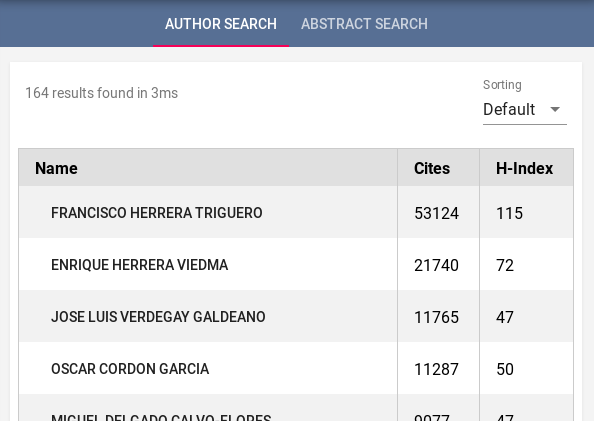
\includegraphics[width=\linewidth]{imagenes/UIAuthor}
	\caption{Búsqueda de autores}
\end{figure}



\newpage
A la derecha de la vista de autores, nos encontramos un menú de selección de ordenamiento que dispone de las opciones que pueden verse en la imagen siguiente y han sido aclaradas en el apartado de desarrollo.


\begin{figure}[h]

	\centering
	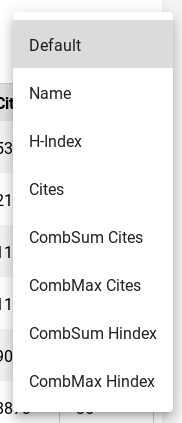
\includegraphics[width=0.20\linewidth]{imagenes/UIAuthorSelection}
	\caption{Ordenación de autores}

\end{figure}


Al seleccionar un autor haciendo click en su nombre se despliega un diálogo donde se nos muestra sus detalles, como se puede ver a continuación. Dicho diálogo contiene botones para acceder a otros perfiles del autor.
\begin{figure}[h]
		  %\vspace{-5pt}
	\centering
	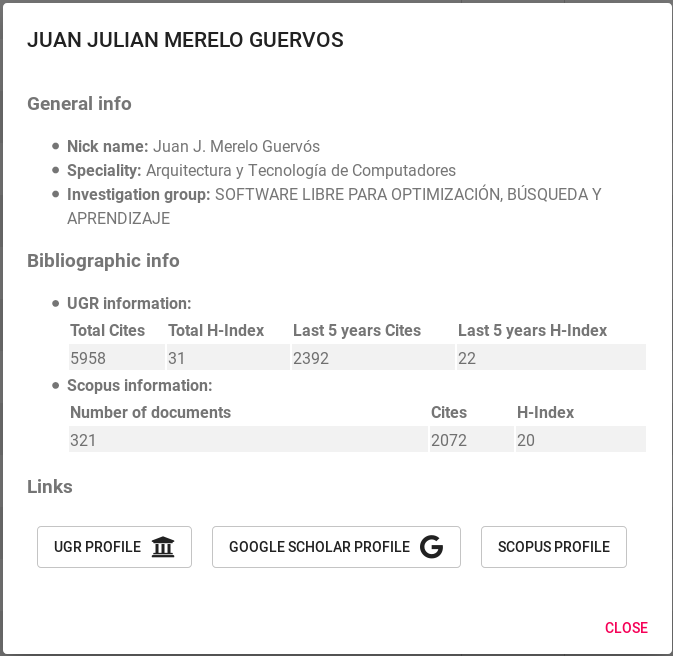
\includegraphics[width=0.7\linewidth]{imagenes/UIAuthorDetail}
	\caption{Vista en detalle de un autor}
	  \vspace{-30pt}
\end{figure}

\section{Búsqueda de artículos}
Este otro módulo, que permite la búsqueda de artículos, cuenta con una interfaz similar, salvo que en lugar de una tabla nos encontramos una lista. Cada elemento representa un artículo y muestra su título, autores, fecha de publicación, número de citas en Scopus y palabras clave si están disponibles.

Cabe destacar que mientras que en la búsqueda de autores se realiza la búsqueda mientras se va escribiendo la petición en el cuadro de búsqueda, en los artículos debido a su mayor número y tamaño es necesario pulsar \texttt{Enter} para lanzar la consulta.
\begin{figure}[h]
	
	\centering
	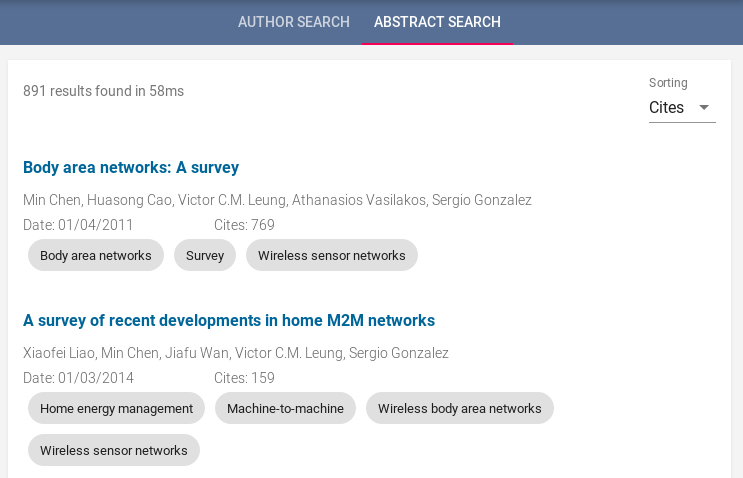
\includegraphics[width=\linewidth]{imagenes/UIAbstract}
	\caption{Búsqueda de artículos}
\end{figure}

\newpage
Al igual que en los autores también disponemos de un menú de selección de ordenación muy similar y con las opciones descritas en desarrollo.

\begin{figure}[h]
	
	\centering
	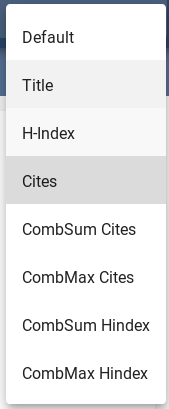
\includegraphics[width=0.20\linewidth]{imagenes/UIAbstractSelection}
	\caption{Ordenación de artículos}
	
\end{figure}

\newpage
Seleccionando alguno de los artículos pasamos a la vista detallada de los mismos, donde vemos una ficha con más datos, un desplegable que muestra el resumen del mismo, un botón para abrirlo en Scopus y las referencias del mismo a otros artículos de la colección (en caso de existir alguna).

\begin{figure}[h]
	%\vspace{-5pt}
	\centering
	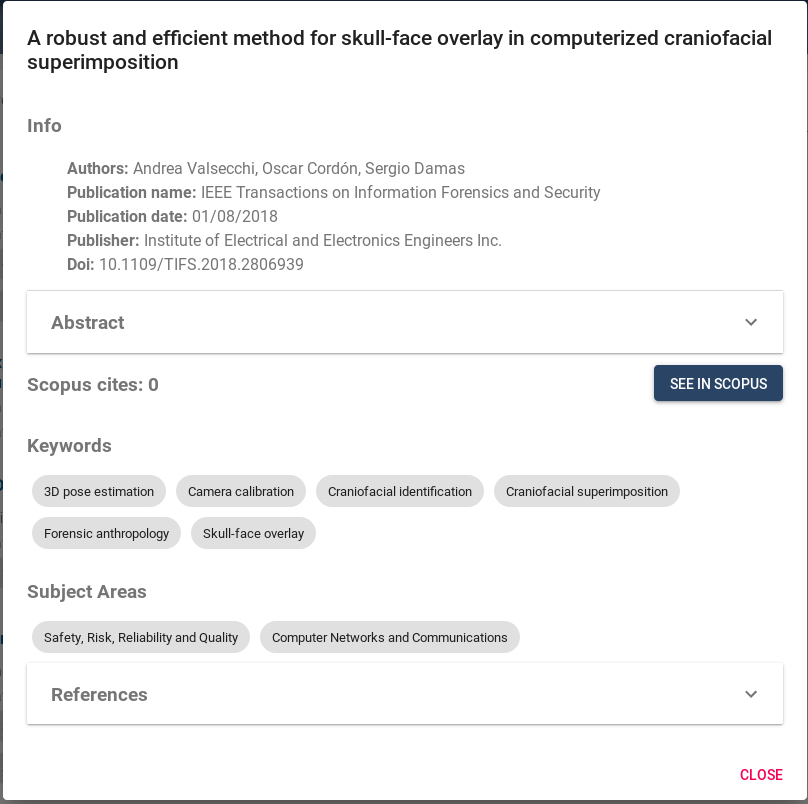
\includegraphics[width=\linewidth]{imagenes/UIAbstractDetail}
	\caption{Vista en detalle de un artículo}
	\vspace{-30pt}
\end{figure}
%%\input{apendices/paper/paper}
%\newglossaryentry{latex}
{
	name=latex,
	description={Is a mark up language specially suited for 
		scientific documents}
}
\newacronym{RI}{RI}{Recuperación de Información}
% \addcontentsline{toc}{chapter}{Glosario}
% \printglossary
\chapter*{}
\thispagestyle{empty}

\end{document}
